%============================================================
\section{Nombre: Manotazo.} \label{hab.Manotazo}
\subsection{Descripción}
El enemigo estrella su mano en el suelo, provocando una onda de piedras en el suelo. El avance de las piedras se hará de manera horizontal. Las piedras infringirán disminuirán la barra de vida del jugador al hacer contacto con el. Después de un tiempo las piedras desaparecerán.
\subsection{Portador}
Itztlacoliuhqui (ver apartado \ref{per:itztlacoliuhqui}).
\subsection{Esquema}
			Ver figura \ref{fig:manotazo}.
			\begin{figure}
				\centering
				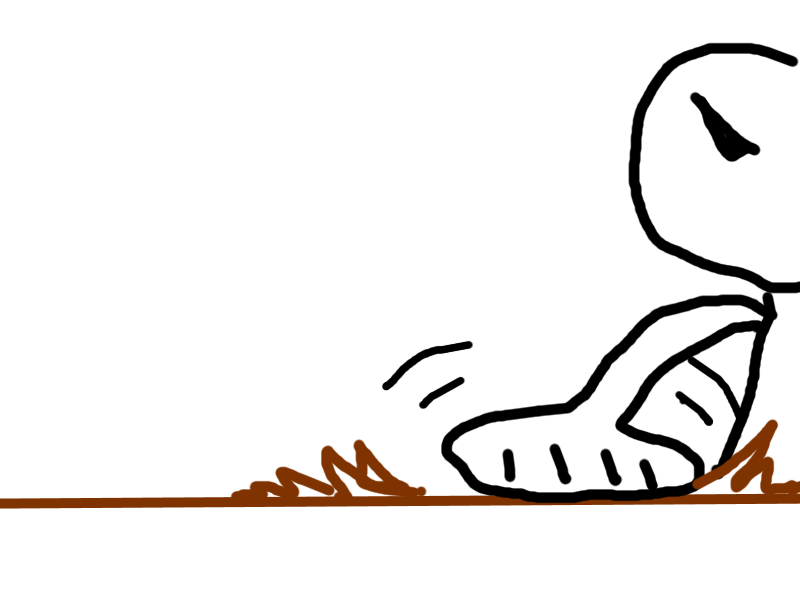
\includegraphics[height=0.2 \textheight]{Imagenes/manotazo}
				\caption{Manotazo.}
				\label{fig:manotazo}
			\end{figure}